\subsection{Dataset}
There is not much real dataset for this topic since transactions data is a sensitive information. Therefore I decided to choose a synthetic dataset GENERATED by a program called PaySim, which is a mobile money transactions simulator. The simulator was developed based on a sample of real transactions extracted from one month of financial logs from a mobile money service implemented in an African country. The original logs were provided by a multinational company, who is the provider of the mobile financial service which is currently running in more than 14 countries all around the world. 

\begin{figure}
  \centering
  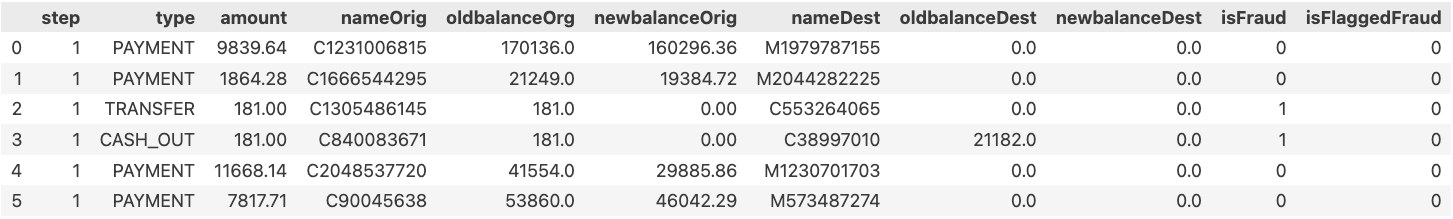
\includegraphics[width=\linewidth]{body/02_methodology/img/figure1.png}
  \caption{Fist 06 rows of the dataset}
\end{figure}

Data we have include both numerical and categorical data, and some of them are not useful for our analysis. Therefore, we need to do some data cleaning and feature engineering to make the data more suitable for our analysis.